\documentclass[english,serif,mathserif,xcolor=pdftex,dvipsnames,table]{beamer}
\usepackage{gc3}

\title[GC3Pie basics]{%
  Basic GC3Pie programming
}
\author[Riccardo Murri]{%
  GC3: Grid Computing Competence Center, \\
  University of Zurich
}
\date{Oct.~1, 2012}

\begin{document}

% title frame
\maketitle

\begin{frame}
  \frametitle{The basic purpose of GC3Pie}

  Run commands.

  \+ 
  Just like the terminal, except GC3Pie can run them on
  \emph{remote} computing resources.

  \+
  (And it can run large collections of commands, but that's for later.)
  
\end{frame}


\begin{frame}
  \frametitle{Specifying commands to run, I}
  
  You need to ``describe'' an application to GC3Pie, in order for
  GC3Pie to use it.

  \+ 
  This ``description'' is a blueprint from which many actual
  command instances can be created.

  \+
  (A few such ``descriptions'' are already part of the core library.)
\end{frame}


\begin{frame}
\frametitle{GC3Libs application model}

  An application is a subclass of the \texttt{gc3libs.Application} class.

  \+
  At a minimum: provide application-specific command-line invocation.

  \+
  Advanced users can customize pre- and post-processing, react on
  state transitions, set computational requirements based on input
  files, influence scheduling.  (This is standard OOP: subclass and
  override a method.)
\end{frame}

\begin{frame}[fragile]
\frametitle{A basic example, I}

  This runs \texttt{expr $x$ * $x$} and saves its output into the file \texttt{stdout.txt}

  \+
\begin{lstlisting}
class SquareApplication(Application):
  """Compute the square of an integer, remotely."""
  def __init__(self, x):
    self.to_square = x
    Application.__init__(
      self,
      arguments=[
        '/usr/bin/expr', 
        x, '*', x],
      inputs=[ ],
      outputs=[ ],
      output_dir='squares.d',
      stdout="stdout.txt",
      join=True)
\end{lstlisting}
\end{frame}


\begin{frame}[fragile]
\frametitle{Always inherit from Application}

  Your application class must inherit from class \texttt{gc3libs.Application}
  \+
\begin{lstlisting}
from gc3libs import Application
class SquareApplication@\HL{(Application)}@:
  def __init__(self, x):
    self.to_square = x
    Application.__init__(
      self,
      arguments=[
        '/usr/bin/expr', 
        x, '*', x],
      inputs=[ ],
      outputs=[ ],
      output_dir='squares.d',
      stdout="stdout.txt",
      join=True)
\end{lstlisting}
\end{frame}


\begin{frame}[fragile]
\frametitle{A basic example, III}

  Perform application-specific initialization first...
  \+
\begin{lstlisting}
class SquareApplication(Application):
  def __init__(self, x):
    @\HL{\textbf{self}.to\_square = x}@
    Application.__init__(
      self,
      arguments=[
        '/usr/bin/expr', 
        x, '*', x],
      inputs=[ ],
      outputs=[ ],
      output_dir='squares.d',
      stdout="stdout.txt",
      join=True)
\end{lstlisting}
\end{frame}

\begin{frame}[fragile]
\frametitle{A basic example, IV}

  ...but remember to call the \lstinline|Application| constructor!
  \+
\begin{lstlisting}
class SquareApplication(Application):
  def __init__(self, x):
    self.to_square = x
    @\HL{Application.\_\_init\_\_(}@
      self,
      arguments=[
        '/usr/bin/expr', 
        x, '*', x],
      inputs=[ ],
      outputs=[ ],
      output_dir='squares.d',
      stdout="stdout.txt",
      join=True)
\end{lstlisting}
\end{frame}

\begin{frame}[fragile]
\frametitle{The \texttt{arguments} parameter, I}

  First, give the list of program arguments.

  \+
\begin{lstlisting}
class SquareApplication(Application):
  def __init__(self, x):
    self.to_square = x
    Application.__init__(
      self,
      @\HL{arguments=[}@
        @\HL{'/usr/bin/expr',}@
        @\HL{x, '*', x}@],
      inputs=[ ],
      outputs=[ ],
      output_dir='squares.d',
      stdout="stdout.txt",
      join=True)
\end{lstlisting}
\end{frame}

\begin{frame}[fragile]
\frametitle{The \texttt{arguments} parameter, II}

The first argument in the list is the name or path to the command to run.

  \+
\begin{lstlisting}
class SquareApplication(Application):
  def __init__(self, x):
    self.to_square = x
    Application.__init__(
      self,
      arguments=[
        @\HL{'/usr/bin/expr',}@
        x, '*', x],
      inputs=[ ],
      outputs=[ ],
      output_dir='squares.d',
      stdout="stdout.txt",
      join=True)
\end{lstlisting}
\end{frame}

\begin{frame}[fragile]
\frametitle{The \texttt{arguments} parameter, III}

The rest of the list are arguments to the program, as you would type
them at the shell prompt.

  \+
\begin{lstlisting}
class SquareApplication(Application):
  def __init__(self, x):
    self.to_square = x
    Application.__init__(
      self,
      arguments=[
        '/usr/bin/expr',
        @\HL{x, '*', x}@],
      inputs=[ ],
      outputs=[ ],
      output_dir='squares.d',
      stdout="stdout.txt",
      join=True)
\end{lstlisting}
\end{frame}


\begin{frame}[fragile]
\frametitle{The \texttt{inputs} parameter, I}

The \texttt{inputs} parameter holds a list of files that you want to
\emph{copy} to the location where the command is executed. (Remember:
this might be a remote computer!)

  \+
\begin{lstlisting}
class SquareApplication(Application):
  def __init__(self, x):
    self.to_square = x
    Application.__init__(
      self,
      arguments=[
        '/usr/bin/expr', 
        x, '*', x],
      @\HL{inputs=[ ],}@
      outputs=[ ],
      output_dir='squares.d',
      stdout="stdout.txt",
      join=True)
\end{lstlisting}
\end{frame}


\begin{frame}[fragile]
  \frametitle{The \texttt{inputs} parameter, II}

  Input files retain their name during the copy.

  \+
  For example:
  \begin{lstlisting}
    inputs = [
      '/home/rmurri/values.dat',
      '/home/rmurri/stats.csv',
      ]
  \end{lstlisting}
  will make files \emph{values.dat} and \emph{stats.csv} available in
  the command execution directory.

\end{frame}


\begin{frame}[fragile]
\frametitle{The \texttt{outputs} parameter, I}

The \texttt{outputs} argument list files that should be copied from
the command execution directory back to your computer.

  \+
\begin{lstlisting}
class SquareApplication(Application):
  def __init__(self, x):
    self.to_square = x
    Application.__init__(
      self,
      arguments=[
        '/usr/bin/expr', 
        x, '*', x],
      inputs=[ ],
      @\HL{outputs=[ ],}@
      output_dir='squares.d',
      stdout="stdout.txt",
      join=True)
\end{lstlisting}
\end{frame}


\begin{frame}[fragile]
  \frametitle{The \texttt{inputs} parameter, II}

  Output file names are \emph{relative to the execution directory}.
  For example:
  \begin{lstlisting}
    outputs = [ 'result.dat', 'program.log' ]
  \end{lstlisting}

  \+ 
  (Contrast with input files, which must be specified by
  \emph{absolute path}, e.g., \texttt{/home/rmurri/values.dat})

  \+ 
  Any file with the given name that is found in the execution
  directory will be copied back. (\emph{Where?} See next slides!)

  \+ 
  If an output file is \emph{not} found, this is \emph{not} an
  error. In other words, output files are optional.

\end{frame}


\begin{frame}[fragile]
\frametitle{The \texttt{output\_dir} parameter, I}

The \lstinline|output_dir| parameter specifies where output filess
will be downloaded.

\+
\begin{lstlisting}
class SquareApplication(Application):
  def __init__(self, x):
    self.to_square = x
    Application.__init__(
      self,
      arguments=[
        '/usr/bin/expr', 
        x, '*', x],
      inputs=[ ],
      outputs=[ ],
      @\HL{output\_dir='squares.d',}@
      stdout="stdout.txt",
      join=True)
\end{lstlisting}
\end{frame}


\begin{frame}[fragile]
  \frametitle{The \emph{output\_dir} parameter, II}
  
  By default, GC3Pie does not overwrite an existing output directory:
  it will move the existing one to a backup name.

  \+
  So, if \texttt{squares.d} already exists, GC3Pie will:
  \begin{enumerate}
  \item rename it to \lstinline|squares.d.~1~|
  \item create a new directory \texttt{squares.d}
  \item download output files into the new directory
  \end{enumerate}
\end{frame}


\begin{frame}[fragile]
\frametitle{The \texttt{stdout} parameter}

This specifies that the command's \texttt{standard output} should be
saved into a file named \texttt{stdout.txt} and retrieved along with
the other output files.

  \+
\begin{lstlisting}
class SquareApplication(Application):
  def __init__(self, x):
    self.to_square = x
    Application.__init__(
      self,
      arguments=[
        '/usr/bin/expr', 
        x, '*', x],
      inputs=[ ],
      outputs=[ ],
      output_dir='squares.d',
      @\HL{stdout="stdout.txt",}@
      join=True)
\end{lstlisting}
\end{frame}


\begin{frame}[fragile]
\frametitle{(The \texttt{stderr} parameter)}

There's a corresponding \texttt{stderr} option for the command's
\emph{standard error} stream.

  \+
\begin{lstlisting}
class SquareApplication(Application):
  def __init__(self, x):
    self.to_square = x
    Application.__init__(
      self,
      arguments=[
        '/usr/bin/expr', 
        x, '*', x],
      inputs=[ ],
      outputs=[ ],
      output_dir='squares.d',
      @\HL{stdout="stdout.txt",}@
      join=True)
\end{lstlisting}
\end{frame}


\begin{frame}[fragile]
\frametitle{The \texttt{join} parameter}

This specifies that \emph{stdout} and \emph{stderr} should be merged
into one single file (like happens on the terminal screen).

\+
The default is \emph{not} to join, i.e., keep \emph{stdout} and \emph{stderr} separate.

\+
\begin{lstlisting}
class SquareApplication(Application):
  def __init__(self, x):
    self.to_square = x
    Application.__init__(
      self,
      # ...
      outputs=[ ],
      output_dir='squares.d',
      stdout="stdout.txt",
      @\HL{join=True})
\end{lstlisting}
\end{frame}


\begin{frame}
  \begin{center}
    Now that we have an application,
    \\
    what do we do with it?
  \end{center}
\end{frame}


\begin{frame}
\frametitle{A simple high-throughput script structure}

This is the prototypical structure of a script for running jobs on
remote computational resources.

\+
\begin{enumerate}
\item Initialize computational resources
\item Prepare files for submission
\item Submit jobs
\item Monitor job status (loop)
\item Retrieve results
\item Postprocess and display
\end{enumerate}
\end{frame}


\begin{frame}[fragile]
\frametitle{Core operations}

GC3Pie provides a \texttt{Core} object to submit a job, update its
state, retrieve (a snapshot of) the output, or cancel the job.

\+
Core operations are \textbf{blocking}.

\end{frame}


\begin{frame}[fragile]
  \frametitle{How to create a \texttt{Core} instance}
  An instance of core is created with the following two-liner, which
  reads the default configuration file and initializes the
  computational resources:
\begin{lstlisting}
  cfg = gc3libs.config.Configuration(
    *gc3libs.Default.CONFIG_FILE_LOCATIONS,
    auto_enable_auth=True)
  core = gc3libs.core.Core(cfg)
\end{lstlisting}

\+ 
Likely, you will only ever need no more than \emph{one single}
instance of \texttt{Core} in your scripts.

\+
\begin{references}
  \url{http://gc3pie.readthedocs.org/en/latest/gc3libs/api.html#module-gc3libs.config}
\end{references}
\end{frame}


\begin{frame}[fragile]
\frametitle{Core operations: verb/object interface}

\texttt{Core} instances operate on \texttt{Application} instances:
\begin{itemize}
\item submit: \texttt{core.submit(app)}
\item monitor: \texttt{core.update\_state(app)}
\item fetch output: \texttt{core.fetch\_output(app, dir)} (starts working as soon as
    application is RUNNING)
\item cancel job: \texttt{core.kill(app)}
\item free remote resources: \texttt{core.free(app)}
\end{itemize}

\+
\begin{references}
  \url{http://gc3pie.readthedocs.org/en/latest/gc3libs/api.html#gc3libs.core.Core}
\end{references}
\end{frame}

\begin{frame}[fragile]
\frametitle{Application lifecycle}

\texttt{Application} objects can be in one of several states.
\+
\begin{center}
  
\includegraphics[width=0.8\textwidth]{fig/states}
\end{center}
\+
The current state is stored in the \texttt{.execution.state} instance attribute.

\+
\begin{references}
  \url{http://gc3pie.readthedocs.org/en/latest/gc3libs/api.html#gc3libs.Run.state}
\end{references}
\end{frame}

\begin{frame}[fragile]
\frametitle{Application lifecycle: state NEW}
\begin{columns}[c]
  \begin{column}{0.5\textwidth}
    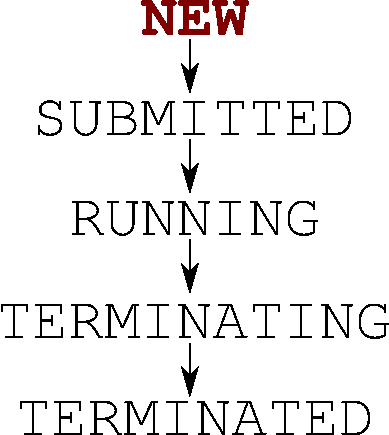
\includegraphics[height=0.7\textheight]{fig/state-NEW}
  \end{column}
  \begin{column}{0.4\textwidth}
    \raggedleft

  \textbf{NEW} is the state of ``just created'' Application objects.
  
  \+ 
  The Application has not yet been sent off to a compute resource:
  it only exists locally.
  \end{column}
\end{columns}
\end{frame}


\begin{frame}[fragile]
\frametitle{Application lifecycle: state SUBMITTED}
\begin{columns}[c]
  \begin{column}{0.5\textwidth}
    
\includegraphics[height=0.7\textheight]{fig/state-SUBMITTED}
  \end{column}
  \begin{column}{0.4\textwidth}
    \raggedleft

    \emph{SUBMITTED} applications have been successfully sent to a
    computational resource.

    \+ 
    (The transition to \emph{RUNNING} happens automatically, as we
    do not control the remote execution.)
  \end{column}
\end{columns}
\end{frame}


\begin{frame}[fragile]
\frametitle{Application lifecycle: state RUNNING}
\begin{columns}[c]
  \begin{column}{0.5\textwidth}
    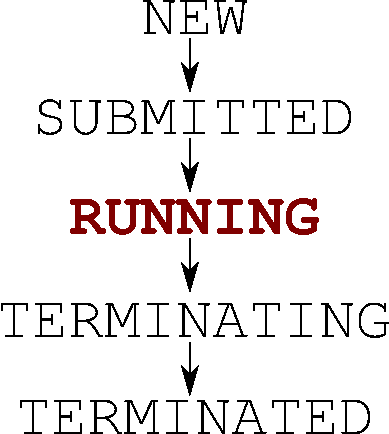
\includegraphics[height=0.7\textheight]{fig/state-RUNNING}
  \end{column}
  \begin{column}{0.4\textwidth}
    \raggedleft

    \emph{RUNNING} state happens when the computational job associated to an
    application starts executing on the computational resource.
  \end{column}
\end{columns}
\end{frame}


\begin{frame}[fragile]
\frametitle{Application lifecycle: state TERMINATING}
\begin{columns}[c]
  \begin{column}{0.5\textwidth}
    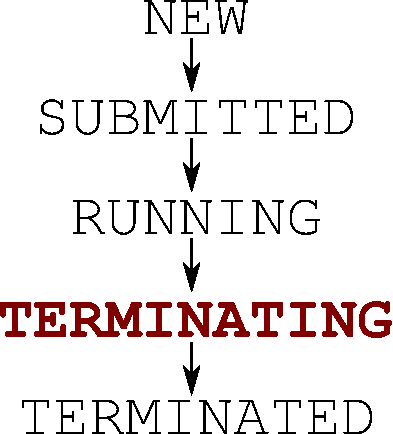
\includegraphics[height=0.7\textheight]{fig/state-TERMINATING}
  \end{column}
  \begin{column}{0.4\textwidth}
    \raggedleft

    \emph{TERMINATING} state when a computational job has finished
    running, for whatever reason.

    \+
    (Transition to \emph{TERMINATED} only happens when \texttt{fetch\_output} is called.)
  \end{column}
\end{columns}
\end{frame}


\begin{frame}[fragile]
\frametitle{Application lifecycle: state TERMINATED}
\begin{columns}[c]
  \begin{column}{0.5\textwidth}
    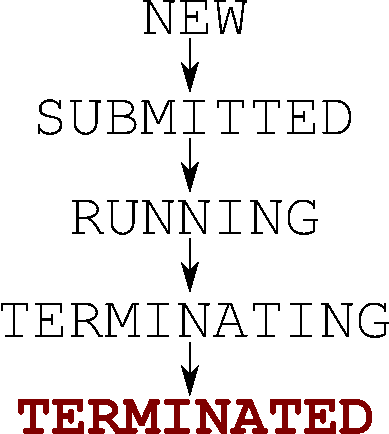
\includegraphics[height=0.7\textheight]{fig/state-TERMINATED}
  \end{column}
  \begin{column}{0.4\textwidth}
    \raggedleft

    A job is \emph{TERMINATED} when its final output has been
    retrieved and is available locally.

    \+ 
    The exit code of \emph{TERMINATED} jobs can be inspected to
    find out whether the termination was successful or unsuccessful,
    or if the program was forcibly ended.

  \end{column}
\end{columns}
\end{frame}


\begin{frame}[fragile]
\frametitle{A successful run or not?}

  There's a \emph{single TERMINATED state}, whatever the job outcome.

  \+ 
  You have to inspect the exit code and signals to determine the
  cause of ``job death''.

  \+ 
  The \texttt{.execution.exitcode} instance attribute holds the
  numeric exitcode of the executed command, or \texttt{None} if the
  command has not finished running yet.
  
  \+ 
  The \texttt{.execution.signal} instance attribute is non-zero if
  the program was killed by a signal (e.g., memory error / segmentation fault).
\end{frame}


\begin{frame}[fragile]
\frametitle{Application lifecycle: error states}
\begin{columns}[c]
  \begin{column}{0.5\textwidth}
    
\includegraphics[width=\textwidth]{fig/states-error}
  \end{column}
  \begin{column}{0.5\textwidth}
    \raggedleft

    Two jobs indicate an error state, i.e., impossibility to carry a
    job to termination.
  \end{column}
\end{columns}

\+ 
A job is in \emph{STOPPED} state when its execution has been
blocked at the remote site and GC3Pie cannot recover
automatically.  User or sysadmin intervention is required.

\+ 
A job is in \emph{UNKNOWN} state when GC3Pie can no longer
monitor it at the remote site. (As this might be due to network
failures, jobs \emph{can} get out of \emph{UNKNOWN}
automatically.)
\end{frame}


\begin{frame}
\frametitle{A simple high-throughput script, GC3Libs version}

\begin{enumerate}
\item \emph{Create a gc3libs.Core instance}
\item \emph{Create instance(s) of the application class}
\item Submit applications (\texttt{Core.submit})
\item Monitor application status (\texttt{Core.update\_job\_state})
\item Retrieve results (\texttt{Core.fetch\_output})
\item Postprocess and display
\end{enumerate}
\end{frame}


\begin{frame}[fragile]
\frametitle{What about post-processing?}
\label{sec-11}

When the remote computation is done, the \texttt{terminated} method of
the application instance is called.

\+
The path to the output directory is available as \lstinline|self.output_dir|.

\+
\begin{lstlisting}
def terminated(self):
  output_file = open(self.output_dir+'/'+self.stdout)
  output_value = output_file.read()
  self.result = int(output_value)
\end{lstlisting}

\+
The above code sets \lstinline|self.result| to the integer value computed by
running \texttt{expr x * x}.
\end{frame}


\begin{frame}[fragile]
  \frametitle{Putting it all together}
  
  The script
  \href{http://www.gc3.uzh.ch/teaching/gc3pie2012/square.py}{square.py}
  provides an example of how all these work together.
\end{frame}


\begin{frame}
  \begin{exercise}
    Copy the
    \href{http://www.gc3.uzh.ch/teaching/gc3pie2012/square.py}{square.py}
    script to a file \texttt{cpuinfo.py} and modify it to run the
    command \texttt{cat /proc/cpuinfo} instead of squaring a number.
    Run it and verify that it gave correct information about your computer's CPU.
  \end{exercise}

  \+
  \begin{exercise}
    Modify the \texttt{cpuinfo.py} script from the previous exercise,
    and add a post-processing method to extract the CPU model
    information and print it.  (The CPU model information is in the
    line that starts with ``model name''.)
  \end{exercise}
\end{frame}


\end{document}

%%% Local Variables: 
%%% mode: latex
%%% TeX-master: t
%%% End: 
